\documentclass[11pt,a4paper,fontset=none]{ctexart}
\usepackage{geometry}
\geometry{left=2.5cm,right=2.5cm,top=2.6cm,bottom=2.6cm,headheight=16pt}
\usepackage{fontspec}
\setCJKmainfont{Noto Serif CJK SC}[BoldFont=Noto Serif CJK SC]
\setCJKsansfont{Noto Sans CJK SC}[BoldFont=Noto Sans CJK SC]
\setCJKmonofont{Noto Sans Mono CJK SC}
\setmonofont{DejaVu Sans Mono}[Scale=0.9]
\setlength{\emergencystretch}{3em}
\usepackage{booktabs}
\usepackage{tabularx}
\usepackage{longtable}
\usepackage{array}
\usepackage{graphicx}
\usepackage{float}
\usepackage{caption}
\usepackage{enumitem}
\usepackage{setspace}
\usepackage{xcolor}
\usepackage{fancyhdr}
\usepackage{titlesec}
\usepackage{listings}
\usepackage[hidelinks]{hyperref}

\linespread{1.5}
\setlength{\parskip}{0.2em}
\setlength{\parindent}{2em}

\ctexset{
  section={format={\sffamily\bfseries\zihao{4}}, aftername={\quad}, beforeskip={1.6ex plus 0.4ex}, afterskip={1.1ex}},
  subsection={format={\sffamily\bfseries\zihao{-4}}, aftername={\quad}, beforeskip={1.2ex plus 0.3ex}, afterskip={0.8ex}},
  subsubsection={format={\sffamily\bfseries\zihao{5}}, aftername={\quad}},
}

\renewcommand{\topfraction}{0.92}
\renewcommand{\bottomfraction}{0.85}
\renewcommand{\textfraction}{0.06}
\renewcommand{\floatpagefraction}{0.80}
\setcounter{topnumber}{3}
\setcounter{bottomnumber}{2}
\setcounter{totalnumber}{4}

\captionsetup{font=small,labelfont=normalfont,labelsep=quad,skip=6pt}
\graphicspath{{shots/}{../../实验2_241880332_张洋/UML/}}

\lstset{
  basicstyle=\ttfamily\small,
  breaklines=true,
  frame=none,
  backgroundcolor=\color{gray!6},
  columns=fullflexible,
  keepspaces=true,
  showstringspaces=false,
  xleftmargin=1.2em,
  xrightmargin=0.6em,
  aboveskip=0.9em,
  belowskip=0.9em,
}

\pagestyle{fancy}
\fancyhf{}
\fancyhead[L]{\zihao{5}\sffamily 酒店预订系统 · 实验三 软件实现与构建}
\fancyhead[R]{\zihao{5}\sffamily 241880332 张洋}
\fancyfoot[C]{\zihao{5}\thepage}
\renewcommand{\headrulewidth}{0.4pt}

\begin{document}

\begin{titlepage}
\centering
\vspace*{3cm}
{\sffamily\zihao{5} 软件设计与建模\quad 实验报告（三）}\\[2.2em]
{\sffamily\bfseries\zihao{2} 酒店预订系统的软件实现与构建}\\[1.2em]
{\sffamily\zihao{4} 基于实验二 UML 模型的分层实现、大模型辅助与 Git 管理}\\[4cm]
\zihao{4}
\begin{tabular}{rl}
项目名称 & 酒店预订系统 \\
学\quad 号 & 241880332 \\
姓\quad 名 & 张洋 \\
实验日期 & 2026 年 11 月 11 日 \\
\end{tabular}
\vfill
{\zihao{5} 实现依据：实验一需求基线 REQ-001 至 REQ-021，实验二 UML 设计模型}
\end{titlepage}

\thispagestyle{empty}
\tableofcontents
\clearpage

\section{实验任务与完成情况}

\subsection{任务要求}

本次实验要求把实验二中设计的 UML 模型实现为可运行的程序，并完成构建、测试与版本管理。任务书列出的硬性要求有四条：按 UML 图实现代码，且实现的代码量超过 1500 行（图形界面工具自动生成的代码不计入）；遵守所选语言的 Google 风格指南，并用相应工具检测；使用大模型辅助开发，并记录使用过程；用 Git 建立本地仓库并托管到远程仓库。此外还要求借助编译器或 IDE 实际编译、运行程序，报告需说明 UML 到代码的转换方式、源码规模、大模型的辅助方式与生成不符预期时的处理办法。

本实验选用 Python 3.12 与标准库 \texttt{sqlite3}，实现一个命令行界面的酒店预订系统，不引入任何第三方运行时依赖。选择 Python 的理由是：实验二的设计是分层单体，核心难点在事务一致性与并发控制，而不是界面表现；Python 的类型注解与数据类能让“每个 UML 类对应一个代码类”的映射关系保持清晰，而 \texttt{sqlite3} 的 \texttt{BEGIN IMMEDIATE} 可以真实地表达“预订、库存、日志在同一事务内提交”。实验三允许图形界面但并未强制要求，因此界面层采用命令行，把工作量集中在业务规则与数据一致性上。

\subsection{完成情况}

\begin{table}[H]
\centering
\caption{任务要求与完成情况对照}
\small
\begin{tabularx}{\textwidth}{p{4.3cm}p{6.0cm}p{4.0cm}}
\toprule
任务要求 & 交付物 & 状态 \\
\midrule
按 UML 实现代码 & \texttt{hotel\_booking/} 五个分层包，22 个源文件 & 完成 \\
代码量超过 1500 行 & 物理行 3706 行，有效代码行 3055 行 & 完成 \\
遵守 Google Python 风格 & \texttt{pylintrc}，pylint 评分 10.00/10 & 完成 \\
大模型辅助并记录 & 第 \ref{sec:llm} 节，含四个真实的返工案例 & 完成 \\
编译并运行 & \texttt{compileall} 全量通过，\texttt{demo.py} 十三个场景 & 完成 \\
Git 本地与远程仓库 & 已推送至 GitHub 远程仓库 & 完成 \\
单元测试 & 68 个用例，含 20 线程并发抢房 & 完成 \\
\bottomrule
\end{tabularx}
\end{table}

\section{设计输入：实验二的模型}

实现直接沿用实验二产出的四类模型：包图定义了分层，两张类图定义了类与职责，状态图定义了预订的生命周期，时序图定义了“创建预订”这一次交互中各对象的协作顺序。实验三允许实现与设计不一致，但本次实现尽量保持了一致，只在数据访问的具体写法上（例如用条件更新代替 UML 中较抽象的“扣减库存”操作）做了细化。

\begin{figure}[htbp]
\centering
\includegraphics[width=0.92\textwidth]{UML包图.png}
\caption{实验二的包图：界面层、应用层、服务层、数据访问层与领域层}
\end{figure}

按照包图，代码目录与包一一对应，依赖方向严格单向：

\begin{lstlisting}
hotel_booking/
  domain/    纯业务规则：枚举、实体、状态机、日期与金额校验、错误
  data/      SQLite 访问：表结构、连接与事务、仓储、种子数据
  service/   用例编排与事务边界：认证、日志、库存、预订、酒店、统计
  api/       装配层：Application 统一组装服务
  cli/       命令行界面：菜单、输入校验、错误渲染
\end{lstlisting}

\texttt{domain} 不导入其他任何层，因此预订规则、状态机、金额计算可以脱离数据库直接测试；\texttt{data} 是唯一出现 SQL 的地方；\texttt{service} 负责事务边界与权限检查；\texttt{api} 只做装配；\texttt{cli} 只做输入输出。这条依赖链在代码审查时反复核对过：\texttt{service} 中没有任何一处直接拼 SQL，\texttt{cli} 中没有任何一处直接调用仓储。

\section{UML 到代码的转换}

\subsection{类图到类：数据与行为分离}

两张类图分别描述领域实体和服务与数据访问对象。转换时遵循三条规则：类图中的每个类对应一个 Python 类，类名保持一致；类图中的属性对应 \texttt{dataclass} 的字段，并用类型注解固定类型；类图中的操作对应方法，但涉及数据库的操作不放进实体，而是放进仓储类。这样做是因为实体需要在测试中大量构造，一旦带上数据库连接就无法脱离文件系统。

\begin{table}[H]
\centering
\caption{类图元素与代码的对应关系}
\small
\begin{tabularx}{\textwidth}{p{3.5cm}p{4.8cm}p{6.2cm}}
\toprule
UML 元素 & 代码位置 & 转换说明 \\
\midrule
User、Hotel、RoomType & \texttt{domain/entities.py} & \texttt{dataclass(slots=True)}，含 \texttt{is\_bookable} 等自身查询 \\
DailyInventory & 同上 & 每日库存，含 \texttt{sellable\_rooms} 与 \texttt{is\_open} \\
Booking & 同上 & 含 \texttt{nights}、\texttt{dates}、\texttt{is\_active}、\texttt{can\_transit\_to} \\
OperationLog & 同上 & 含 \texttt{masked\_detail}，输出前对手机号脱敏 \\
AuthService & \texttt{service/auth.py} & 注册、登录、\texttt{require\_role}、\texttt{require\_hotel\_scope} \\
BookingService & \texttt{service/booking.py} & 创建、修改、取消、确认、拒绝、入住、退房、超时清扫 \\
InventoryService & \texttt{service/inventory.py} & 每日库存维护、批量设置、停售、多条件查询 \\
HotelService & \texttt{service/hotel.py} & 信息维护、警告、下架、临时停业 \\
StatisticsService & \texttt{service/statistics.py} & 逐日统计与汇总，口径写在模块文档中 \\
LogService & \texttt{service/log.py} & 接收调用方事务连接写日志，\texttt{purge\_expired} 保留 180 天 \\
六个仓储类 & \texttt{data/repositories.py} & 每个聚合根一个仓储，SQL 只出现在这里 \\
SearchRepository & 同上 & 查询用 \texttt{JOIN} 与 \texttt{HAVING} 保证“全程可订” \\
Application & \texttt{api/application.py} & 组装对象图，对外只暴露用例方法 \\
\bottomrule
\end{tabularx}
\end{table}

类图中的关联关系（酒店拥有房型、预订属于顾客）在代码中体现为外键与查询方法，而不是把对象图直接序列化进表。表结构见 \texttt{data/schema.py}：\texttt{hotels}、\texttt{room\_types}、\texttt{inventory}、\texttt{bookings}、\texttt{users}、\texttt{operation\_logs} 六张表，另有唯一索引保证“同房型同日期只有一条库存”与“幂等键唯一”。

\begin{figure}[htbp]
\centering
\includegraphics[width=0.95\textwidth]{UML类图-领域实体.png}
\caption{实验二的领域实体类图（实现中逐类落地）}
\end{figure}

\subsection{状态图到状态机：转换表加条件更新}

预订状态图有五个状态与七条合法迁移。转换时没有写成散落在各服务方法里的 \texttt{if}，而是抽成一张显式的转换表，放在 \texttt{domain/rules.py}：

\begin{lstlisting}
_TRANSITIONS = {
    PENDING_CONFIRM: {CONFIRMED, REJECTED, CANCELLED, TIMEOUT_CANCELLED},
    CONFIRMED:       {CHECKED_IN, CANCELLED},
    CHECKED_IN:      {CHECKED_OUT},
    CHECKED_OUT:     set(),
    CANCELLED:       set(),
    REJECTED:        set(),
    TIMEOUT_CANCELLED: set(),
}
\end{lstlisting}

只有这张表还不够，因为“检查状态”和“改状态”之间存在时间窗口，旧页面正是利用这个窗口覆盖新状态的。因此每次状态变更都写成带旧状态条件的更新：

\begin{lstlisting}
UPDATE bookings SET status = ?, updated_at = ?
WHERE booking_id = ? AND status = ?      -- 旧状态作为条件
\end{lstlisting}

影响行数为 0 就说明状态已被别人改过，此时抛出 \texttt{STATE\_NOT\_ALLOWED}，由界面提示用户刷新。这一条同时满足了 REQ-013（旧页面不覆盖新状态）与 REQ-018（并发下只有一个请求成功）。对于“重复确认”“重复入住”“重复取消”，先判断目标状态是否已等于当前状态，是则直接返回原结果；取消时的库存回补因此只会发生一次。

\subsection{时序图到事务边界：一个方法一个事务}

实验二的创建预订时序图包含“校验日期、逐日查库存、逐日扣减、生成预订、写日志、返回结果”六个步骤。实现时把这六步放进同一个 \texttt{with self.database.transaction()} 代码块，数据库连接在整块内共享：

\begin{lstlisting}
with self._db.transaction() as conn:          # BEGIN IMMEDIATE
    existing = BookingRepository.get_by_key(conn, idempotency_key)
    if existing: return CreateResult(existing, replayed=True)
    stay_prices = self._reserve(conn, room_type, dates, rooms)
    BookingRepository.insert(conn, booking)
    self._logs.write(conn, operator, "BOOKING", ...)   # 同一连接
\end{lstlisting}

事务提交或回滚由上下文管理器统一处理，任何一步抛异常都会回滚全部写入。日志服务刻意不自己开连接，而是接收调用方的事务连接，这样“业务成功但日志失败”在结构上就不可能发生，正是 REQ-020 的要求。

\subsection{活动图到校验顺序}

活动图中的判断菱形被转换为固定的校验顺序，保证用户先看到最相关的错误：日期范围（是否早于今天、是否超过 30 晚）$\rightarrow$ 房型是否存在且在售 $\rightarrow$ 酒店是否可订 $\rightarrow$ 逐日库存是否足够 $\rightarrow$ 写库与写日志。库存不足时不是笼统地提示“失败”，而是区分三种情形：当日停售、已售完、仅剩 N 间不足 M 间，对应 REQ-012 与 REQ-021。

\subsection{源代码规模}

按有效代码行（去掉空行、注释与文档字符串）统计，产品代码合计 3055 行，物理行 3706 行，超过任务要求的 1500 行。单元测试另有 788 行，未计入上表。

\begin{table}[H]
\centering
\caption{源程序规模统计（产品代码）}
\small
\begin{tabular}{lrr}
\toprule
文件 & 物理行 & 有效代码行 \\
\midrule
\texttt{domain/enums.py} & 80 & 48 \\
\texttt{domain/errors.py} & 185 & 148 \\
\texttt{domain/entities.py} & 166 & 112 \\
\texttt{domain/rules.py} & 198 & 157 \\
\texttt{data/schema.py} & 107 & 93 \\
\texttt{data/database.py} & 88 & 57 \\
\texttt{data/repositories.py} & 731 & 609 \\
\texttt{data/seed.py} & 126 & 111 \\
\texttt{service/auth.py} & 224 & 179 \\
\texttt{service/log.py} & 108 & 82 \\
\texttt{service/inventory.py} & 269 & 232 \\
\texttt{service/booking.py} & 569 & 501 \\
\texttt{service/hotel.py} & 305 & 278 \\
\texttt{service/statistics.py} & 183 & 152 \\
\texttt{api/application.py} & 64 & 37 \\
\texttt{cli/app.py} & 295 & 258 \\
各包 \texttt{\_\_init\_\_.py} 合计 & 9 & 1 \\
\midrule
合计 & 3706 & 3055 \\
\bottomrule
\end{tabular}
\end{table}

代码规模主要来自三处：仓储层的 SQL 与字段映射、预订服务的状态机与异常分支、以及错误提示的三段式文案。这三处恰好是需求中最容易漏项的环节，因此没有为了“行数达标”去堆砌无意义的代码。

\section{大模型辅助实现}
\label{sec:llm}

\subsection{协作方式：把“需求到代码”拆成三段}

任务书提醒“可以将需求到代码分解为需求、存根加规约、代码三个阶段”。本次实现按这个思路组织了与大模型的协作，每一段都有明确的人工检查点。

第一段是需求到规约。把实验一的 21 条需求原文贴给大模型，要求它只输出包结构、每个文件要放哪些类、每个类的公开方法签名与文档字符串，不许写实现。这个阶段的产出是一份“骨架加规约”，人工逐条对照需求检查：REQ-013 的幂等要求有没有对应的参数、REQ-020 的日志一致性有没有体现在方法签名里。规约确认后，后续生成的代码才有稳定的约束。

第二段是规约到实现。按文件逐个让大模型补全函数体，并在提示中固定三条约束：只允许使用标准库、遵守 Google Python 风格（80 列、类型注解、完整 docstring）、不得跨层调用。每生成一个文件就立刻运行 \texttt{ast.parse} 与 \texttt{compileall} 检查语法，再人工阅读全部代码。

第三段是自检。让大模型扮演审查者，对已完成的代码提出测试用例清单，再由人工筛选实现。这个阶段最有价值：模型提出的用例里有一部分是“正确但没有覆盖”（例如只测正常退房），人工补上了“未入住直接退房”“重复取消”这类边界；也有一部分用例暴露出实现本身的语义错误（见下文第二例）。

\subsection{让大模型承担的具体工作}

\begin{table}[H]
\centering
\caption{大模型在本实验中的任务分工}
\small
\begin{tabularx}{\textwidth}{p{4.2cm}p{3.6cm}X}
\toprule
任务 & 输入 & 产出与人工处理 \\
\midrule
包与模块划分 & 实验二包图、21 条需求 & 给出五个包与文件清单；人工删除了它顺手加上的“工具模块”，因为该类只有一个函数，合并进 \texttt{rules} \\
类骨架与规约 & 类图两张 & 生成数据类字段与方法签名；人工为 \texttt{Booking} 补了 \texttt{dates} 与 \texttt{is\_active}，类图中有但模型漏掉 \\
仓储与 SQL & 表结构 & 生成六张表的 DDL 与增删改查；人工把“先查后改”的库存扣减改为条件更新 \\
并发控制方案 & REQ-018 & 提出三种方案（悲观锁、条件更新、应用层队列），人工选定条件更新并补写并发测试 \\
状态机与守卫 & 状态图 & 生成转换表；人工补充“目标状态已达成则返回原结果”的短路，保证重复操作幂等 \\
错误提示文案 & REQ-021 & 生成三段式模板与错误码表；人工重写二十余条中文文案，使其符合界面语境 \\
单元测试设计 & 服务层代码 & 提出 40 余条用例；人工筛选、补边界，最终落地 68 条 \\
风格整改 & pylint 报告 & 逐条给出修改建议；人工判断哪些该改、哪些属于误报 \\
\bottomrule
\end{tabularx}
\end{table}

\subsection{生成不符合预期的四种情形及处理}

第一种是结构性问题：包内自引用。模型在生成装配层时，顺手写了一句 \texttt{from hotel\_booking.api import \_\_all\_\_}，让一个包从自己内部导入。这在语法上完全合法，单个文件看也不像错误，但程序一启动就进入循环导入。处理办法是人工删除该行，并把“禁止包内自引用、装配层只允许向下依赖”写进后续提示词。这件事说明语法检查通过不等于结构正确，必须有人读过每一行。

第二种是语义错误：与需求相反。模型把 \texttt{Hotel.is\_bookable} 写成“只有 ONLINE 状态可以预订”，看起来顺理成章，但 REQ-002 中“警告”只是标记问题酒店，并不停止营业。这个错误在人工阅读时没有看出来，是单元测试中“警告状态仍可预订”这一条用例失败后暴露的。修复是把可订状态改为 ONLINE 与 WARNING 两种，并在实体文档字符串里写明依据。这是“测试用例反向校验实现”的典型例子。

第三种是展示层错误：打印了旧对象。演示脚本取消预订后打印 \texttt{cancel\_target.status}，由于实体是不可变快照，打印出来仍是“待确认”。程序逻辑没有问题，但演示结果会误导读者。处理办法是统一约定“以服务方法的返回值为准”，所有打印都使用返回值。

第四种是风格告警：参数过多与重复代码。初版 pylint 评分 9.68，主要告警是 \texttt{too-many-arguments} 与 \texttt{duplicate-code}，集中在日志写入与仓储方法。处理时分了两类：真正的问题（\texttt{no-else-raise}、超长行、未使用的导入）直接修改代码；设计上合理的部分（日志固定字段、实体多字段）在 \texttt{pylintrc} 中放宽阈值或在对应函数上写行内抑制注释，并在注释里说明理由。最终评分 10.00，抑制项在报告中如实列出，而不是把规则整体关掉。

\subsection{人工审查清单}

每接受一段生成代码，都按下面六项检查，任何一项不通过就退回重写：

\begin{enumerate}[leftmargin=2.2em,itemsep=0.2em]
\item 依赖方向：这段代码有没有反向依赖上层，有没有在 \texttt{domain} 中出现 SQL 或文件操作。
\item 事务边界：一次业务操作是否只有一个事务，日志是否使用同一个连接。
\item 并发正确性：库存扣减是否带“可用数量足够”的条件，状态更新是否带旧状态条件。
\item 数据安全：密码是否只以哈希形式出现，日志中是否可能落下明文手机号，SQL 是否全部参数化。
\item 异常处理：是否吞掉了异常，抛出的错误是否带原因、建议与去向。
\item 可读性：命名是否符合 Google 风格，函数是否只做一件事，注释是否解释“为什么”而不是“是什么”。
\end{enumerate}

这套检查的价值在于把“看起来对”变成“知道为什么对”。例如条件更新扣库存这一条，如果不追问“并发时会不会两个事务都读到 1 间”，代码在单线程测试中永远是正确的。

\section{编译与运行}

\subsection{运行环境}

\begin{table}[H]
\centering
\caption{实验环境}
\small
\begin{tabular}{ll}
\toprule
项目 & 版本或说明 \\
\midrule
操作系统 & Linux（x86\_64）\\
解释器 & Python 3.12.11（\texttt{/opt/python3.12/bin/python3}）\\
数据库 & SQLite 3（Python 标准库 \texttt{sqlite3}）\\
运行时依赖 & 无第三方库 \\
开发依赖 & pytest 9.2.0、pylint 4.1.3 \\
构建与配置 & \texttt{pyproject.toml}、\texttt{pylintrc}、\texttt{.gitignore} \\
\bottomrule
\end{tabular}
\end{table}

Python 是解释型语言，没有传统意义上的链接步骤。本次用 \texttt{python3 -m compileall} 对全部模块做字节码编译，语法错误会在这一步暴露；随后直接运行程序。为便于复核，编译检查与运行输出都保存在仓库的 \texttt{docs/} 目录中。

\begin{lstlisting}
$ python3 -m compileall -q hotel_booking tests
$ python3 -m pytest tests -q
68 passed in 7.9s
\end{lstlisting}

\subsection{运行结果}

\texttt{scripts/demo.py} 在一套临时数据库上依次执行十三个场景，覆盖需求基线中的主要验收点：三角色登录、每日库存设置、多条件查询、创建预订与逐日扣减、第二个顾客抢同一间时的精确提示、同一幂等键重复提交、确认与入住退房、取消并回补库存、越权操作被拒、日志写失败整单回滚、统计报表、日志查询与脱敏。图 \ref{fig:run1} 至图 \ref{fig:run3} 是其中十三个场景的实际输出。

\begin{figure}[htbp]
\centering
\begin{minipage}{0.485\textwidth}
\centering
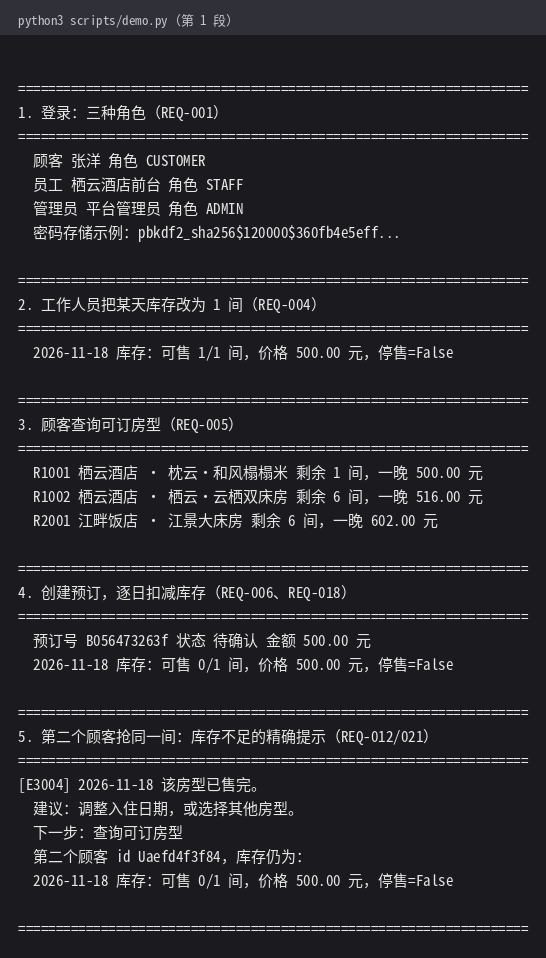
\includegraphics[width=\textwidth]{运行演示1.png}
\caption{运行演示（一）：登录、库存、查询与创建}
\label{fig:run1}
\end{minipage}\hfill
\begin{minipage}{0.485\textwidth}
\centering
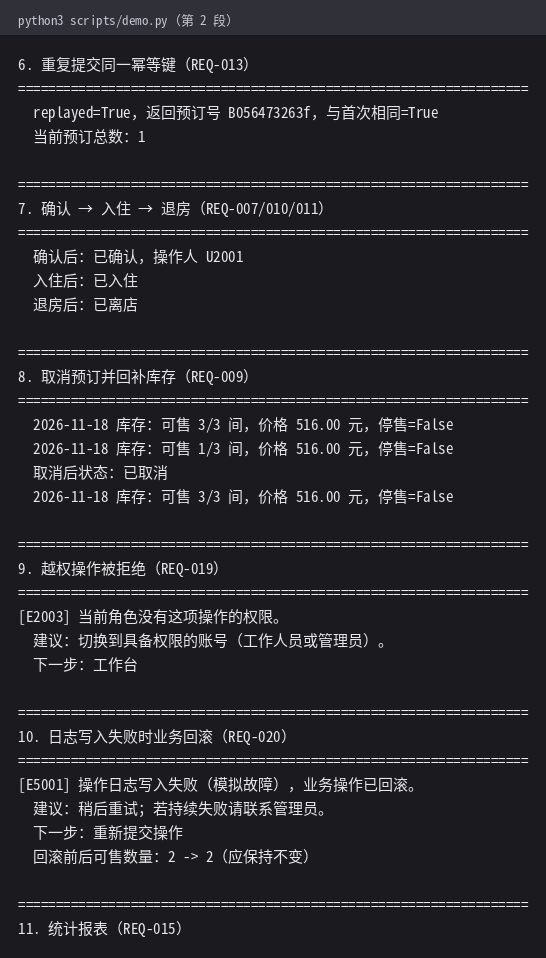
\includegraphics[width=\textwidth]{运行演示2.png}
\caption{运行演示（二）：幂等、流转、取消、越权与回滚}
\label{fig:run2}
\end{minipage}
\end{figure}

\begin{figure}[htbp]
\centering
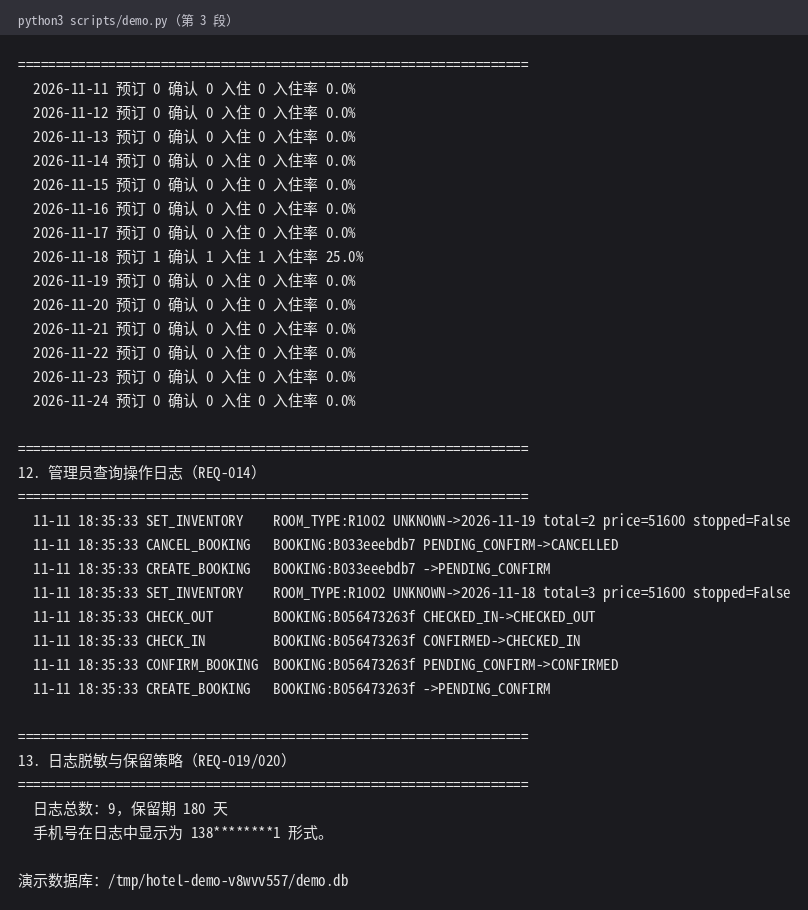
\includegraphics[width=0.68\textwidth]{运行演示3.png}
\caption{运行演示（三）：统计报表与操作日志}
\label{fig:run3}
\end{figure}

其中两个输出值得说明。场景五中第二个顾客看到的不是笼统的“预订失败”，而是“该房型已售完 / 建议调整入住日期，或选择其他房型 / 下一步：查询可订房型”，三段信息分别回答“为什么”“怎么办”“去哪里”，这就是 REQ-021 要的提示。场景八中库存从 3 间降到 1 间、取消后又回到 3 间，说明按晚回补的粒度是对的：两晚的预订各占一间，取消时逐日归还。

\subsection{单元测试}

\begin{table}[H]
\centering
\caption{单元测试分布}
\small
\begin{tabular}{llr}
\toprule
测试文件 & 覆盖内容 & 用例数 \\
\midrule
\texttt{test\_domain.py} & 日期与间数校验、状态机、错误渲染 & 16 \\
\texttt{test\_auth.py} & 注册、登录、密码策略、角色与数据范围 & 9 \\
\texttt{test\_booking.py} & 创建、幂等、修改、取消、确认、入住退房、超时 & 14 \\
\texttt{test\_inventory.py} & 库存唯一性、停售、搜索的四类条件 & 11 \\
\texttt{test\_transaction.py} & 日志回滚、下架联动、脱敏、保留期、停业 & 10 \\
\texttt{test\_statistics.py} & 逐日统计、排除规则、入住率与汇总 & 7 \\
\texttt{test\_concurrency.py} & 20 线程抢最后 1 间 & 1 \\
\midrule
合计 & & 68 \\
\bottomrule
\end{tabular}
\end{table}

并发用例的做法是：把库存设为 1 间，启动 20 个线程，每个线程独立打开数据库连接，用 \texttt{Barrier} 让它们同时发起预订。结果是恰好 1 个线程拿到房间，其余 19 个收到库存不足的错误，最终可售数量为 0 且不为负。这个用例证明条件更新加写锁的组合是有效的，而不是靠“测试时没出错”来判断。

\begin{figure}[htbp]
\centering
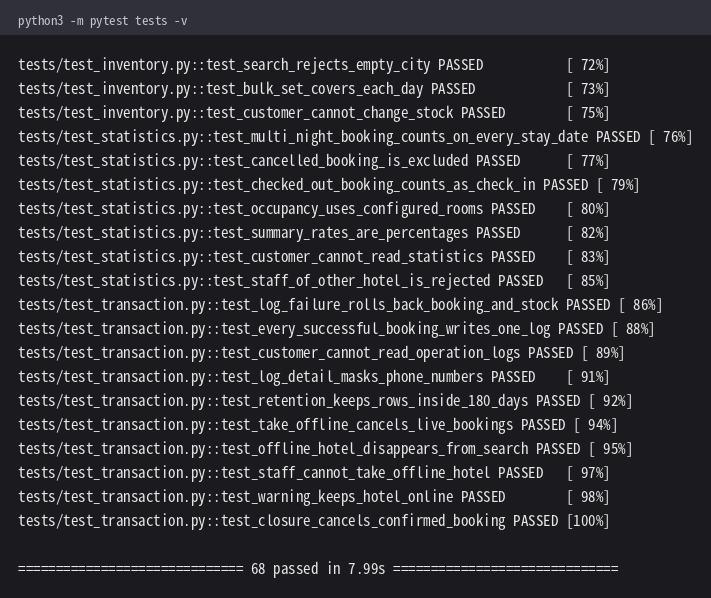
\includegraphics[width=0.72\textwidth]{单元测试.png}
\caption{pytest 运行结果：68 个用例全部通过}
\end{figure}

\subsection{风格检查}

Google Python 风格的主要约束是 80 列行宽、完整的模块与函数文档字符串、清晰的命名、必要的类型注解。用 pylint 检测，配置写在 \texttt{pylintrc} 中，最终评分 10.00/10。

\begin{figure}[htbp]
\centering
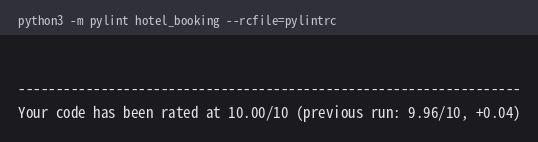
\includegraphics[width=0.78\textwidth]{风格检查.png}
\caption{pylint 风格检查结果：10.00/10}
\end{figure}

配置中只放宽了三类与项目结构有关的阈值，理由都写进了配置文件：实体类与仓储方法天然携带较多字段与参数（\texttt{max-attributes}、\texttt{max-args}）；审计日志在各服务中使用同一套字段模板，重复是刻意的可读性选择（关闭 \texttt{duplicate-code}）；脚本目录不参与库代码评分。其余告警全部通过修改代码消除，包括超长行、多余的 \texttt{else}、未使用的导入、模块内局部导入等。

\section{Git 版本管理}

\subsection{本地仓库}

仓库在项目根目录初始化，主分支为 \texttt{main}，\texttt{.gitignore} 排除了数据库文件、缓存与构建产物，保证提交内容只有源码、测试、文档与配置。提交按“配置、领域层、数据层、服务层、界面层、测试、文档”的顺序拆分，每个提交对应一个可理解的变更单元，便于回溯每一步做了什么。

\begin{table}[H]
\centering
\caption{本地提交历史}
\small
\begin{tabular}{ll}
\toprule
提交 & 内容 \\
\midrule
\texttt{09a063d} & 初始化工程结构与风格检查配置 \\
\texttt{121db7a} & 领域层：实体、枚举、状态机与可行动错误 \\
\texttt{2a5e744} & 数据层：表结构、事务封装、仓储与种子数据 \\
\texttt{735b7f5} & 服务层：认证、日志、库存、预订、酒店与统计 \\
\texttt{18775cc} & 界面层：应用装配与命令行交互 \\
\texttt{8e152ca} & 测试：68 个单元测试与端到端演示脚本 \\
\texttt{8f676d8} & 文档：需求映射与运行说明 \\
\texttt{756ce36} & 文档：实验报告、运行证据与配图脚本 \\
\texttt{303f741} & 文档：调整报告措辞并重新渲染 PDF \\
\bottomrule
\end{tabular}
\end{table}

\begin{figure}[htbp]
\centering
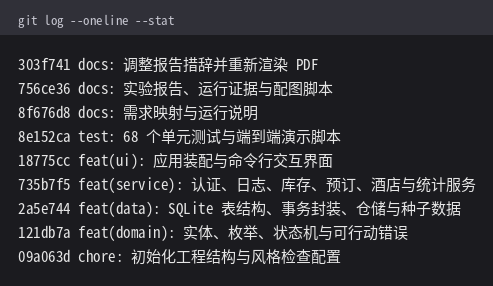
\includegraphics[width=0.72\textwidth]{git日志.png}
\caption{本地仓库的分层提交记录}
\end{figure}

\subsection{远程托管}

远程仓库选择 GitHub 托管，主分支为 \texttt{main}。该仓库此前已用于存放实验一的需求材料，因此推送前先抓取远端分支，再用 \texttt{git rebase origin/main} 把本地九次提交线性接在远端两个已有提交之后：既不覆盖 \texttt{requirement.md} 等既有文件，也避免合并提交造成的平行历史。

\begin{lstlisting}
$ git remote add origin \
    git@github.com:13510703580-eng/hotel-booking-requirements.git
$ git fetch origin && git rebase origin/main
$ git push -u origin main
   e5e3f91..303f741  main -> main
Branch 'main' set up to track remote branch 'main' from 'origin'.
\end{lstlisting}

写权限通过部署密钥授予：在仓库的 Settings 与 Deploy keys 中添加本机公钥并勾选 Allow write access。这种方式只对该仓库有效，实验结束后可在页面上直接删除，不需要提供账号级令牌。推送后远端同时保留实验一的三份材料与本次实现的全部提交历史，仓库首页的文件列表、提交说明与语言统计见图 \ref{fig:github}。

\begin{figure}[htbp]
\centering
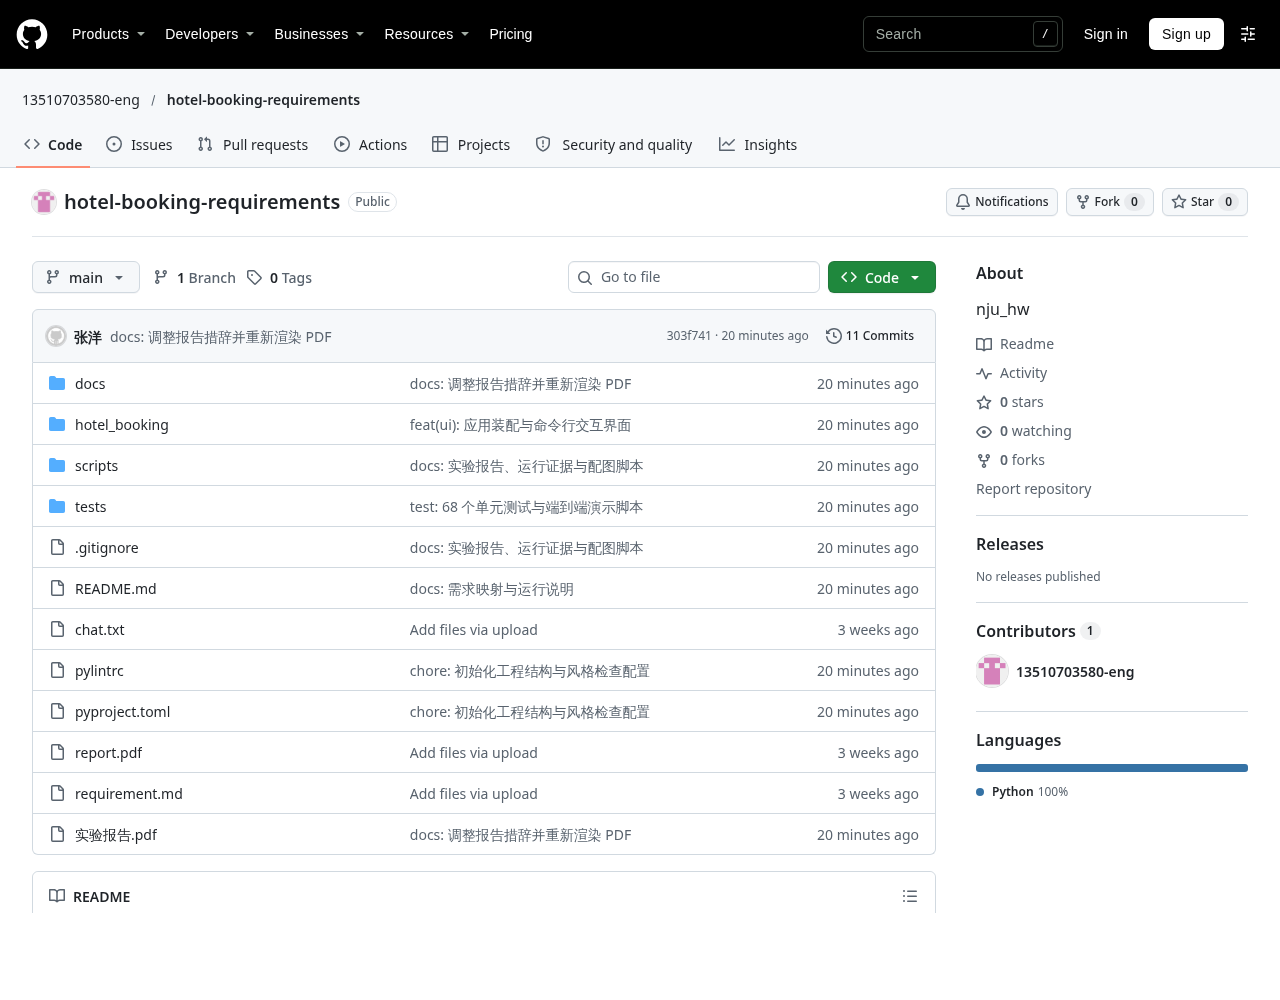
\includegraphics[width=0.95\textwidth]{github仓库.png}
\caption{GitHub 远程仓库：11 次提交、五个目录与语言统计}
\label{fig:github}
\end{figure}

\section{问题与反思}

第一，条件更新比“先查后改”更可靠。最初一版库存扣减是“查剩余数量、够就更新”，单元测试在单线程下全绿，但并发用例一跑就出现超卖。改成带谓词的条件更新后，正确性由数据库的行锁保证，应用层不再需要额外加锁。这个教训直接对应 REQ-018。

第二，日志必须写进业务事务。把日志服务设计成“自己开连接、自己提交”是最容易写出来的版本，但那样一旦日志失败，业务已经提交，数据与审计就对不上。让日志函数接收调用方的连接，是把一致性要求写进接口，而不是写进流程规范。

第三，可行动的错误提示是有成本的。为二十多个错误码各写“原因、建议、去向”，比统一提示“操作失败”多出上百行代码，但这部分恰好是 REQ-021 的验收点。实现时把默认建议放在错误码表里，只有在具体场景更清楚时才覆盖，这样既保证每条错误都有三段信息，又避免在调用处重复写文案。

第四，大模型能显著提速，但不能替代判断。它在结构、命名、样板代码上的产出质量很高，但在“业务语义”上会给出看似合理实则相反的实现，例如把警告状态当成不可订。有效的做法是把需求原文、约束条件和已有接口一起给模型，并要求它先给规约再给代码；同时用测试把语义钉死。凡是没有测试覆盖的语义，最终都要靠人逐行读。

第五，实现与设计的一致性需要主动维护。实验二的状态图没有写“重复确认返回原结果”，实现时补充了这个短路；实验二的类图没有体现幂等键，实现时在表结构里加了唯一索引。这些偏差都记录在本节与代码注释中，如果后续继续迭代，应当回头修订实验二的设计文档。

\begin{thebibliography}{9}
\small
\addcontentsline{toc}{section}{参考文献}
\bibitem{google} Google. Google Python Style Guide[EB/OL]. \url{https://google.github.io/styleguide/pyguide.html}, 2026.
\bibitem{pep8} van Rossum G, Warsaw B, Coghlan A. PEP 8: Style Guide for Python Code[EB/OL]. \url{https://peps.python.org/pep-0008/}, 2001.
\bibitem{pylint} Pylint contributors. Pylint documentation[EB/OL]. \url{https://pylint.readthedocs.io/}, 2026.
\bibitem{sqlite} SQLite Consortium. SQLite Documentation: Transactions and WAL[EB/OL]. \url{https://www.sqlite.org/docs.html}, 2026.
\bibitem{pytest} pytest contributors. pytest documentation[EB/OL]. \url{https://docs.pytest.org/}, 2026.
\bibitem{exp1} 张洋. 酒店预订系统需求分析报告（实验一）[R]. 南京: 软件设计与建模课程, 2026.
\bibitem{exp2} 张洋. 酒店预订系统的软件设计与建模（实验二）[R]. 南京: 软件设计与建模课程, 2026.
\end{thebibliography}

\end{document}
